% Asset ID: A22FurtherKinematicsTikZ-004
% Unit: A22
% Topic: Further Kinematics
% Related section: Projectile motion
\documentclass[tikz,border=8pt]{standalone}
\usepackage{amsmath}
\usetikzlibrary{arrows.meta,positioning,angles,quotes}
\begin{document}

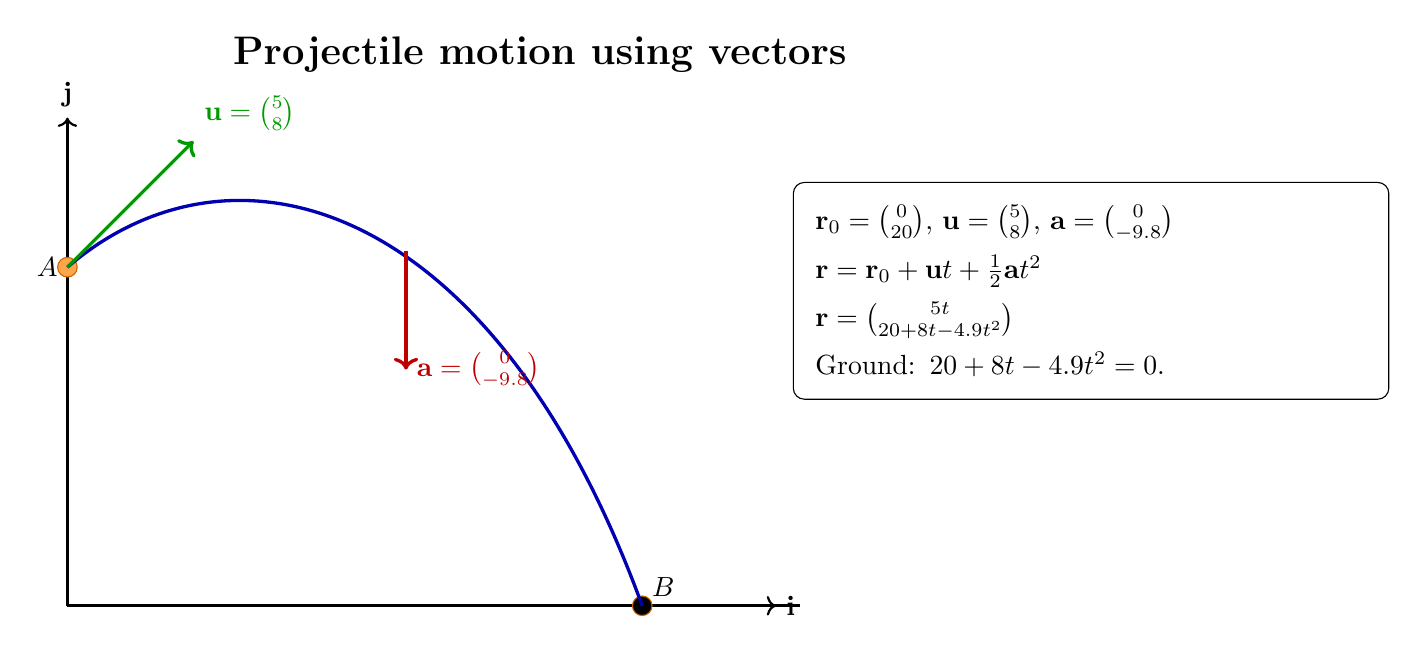
\begin{tikzpicture}[axis/.style={->, thick}, traj/.style={very thick, blue!70!black}, vel/.style={->,very thick,green!60!black}, grav/.style={->,very thick,red!75!black}, point/.style={circle,fill=orange!70,draw=orange!80!black,inner sep=2.5pt}, box/.style={draw,rounded corners,fill=white,align=left,inner sep=8pt}]
\node[font=\bfseries\Large] at (6,7) {Projectile motion using vectors};
\draw[axis] (0,0)--(9,0) node[right] {$\mathbf i$}; \draw[axis] (0,0)--(0,6.2) node[above] {$\mathbf j$}; \draw[very thick] (0,0)--(9.3,0);
\coordinate (A) at (0,4.3); \coordinate (B) at (7.3,0);
\node[point] at (A) {}; \node[left] at (A) {$A$}; \node[point, fill=black] at (B) {}; \node[above right] at (B) {$B$};
\draw[traj] (A)..controls (2.1,6.1) and (5.4,5.2)..(B);
\draw[vel] (A)--++(1.6,1.6) node[above right] {$\mathbf u=\binom{5}{8}$};
\draw[grav] (4.3,4.5)--++(0,-1.5) node[right] {$\mathbf a=\binom{0}{-9.8}$};
\node[box, text width=7cm] at (13,4) {$\mathbf r_0=\binom{0}{20}$, $\mathbf u=\binom{5}{8}$, $\mathbf a=\binom{0}{-9.8}$\\[4pt]$\mathbf r=\mathbf r_0+\mathbf ut+\frac12\mathbf at^2$\\[4pt]$\mathbf r=\binom{5t}{20+8t-4.9t^2}$\\[4pt]Ground: $20+8t-4.9t^2=0$.};
\end{tikzpicture}
\end{document}
